\section{Matériels et Méthodes}

\subsection{Instruments scientifiques utilisés (logiciels, programmes, modèles, etc.)}
Pour cette étude, une combinaison de logiciels et de langages de programmation a été utilisée pour traiter, analyser et calculer l'indice d'upwelling de Bakun (CUI) à partir des données de transport d'Ekman. Les outils scientifiques utilisés incluent :

\begin{itemize}
    \item \textbf{R} : Un environnement de programmation et un logiciel statistique utilisé pour le traitement des données et la création de graphiques.
    
    \begin{figure}[H]
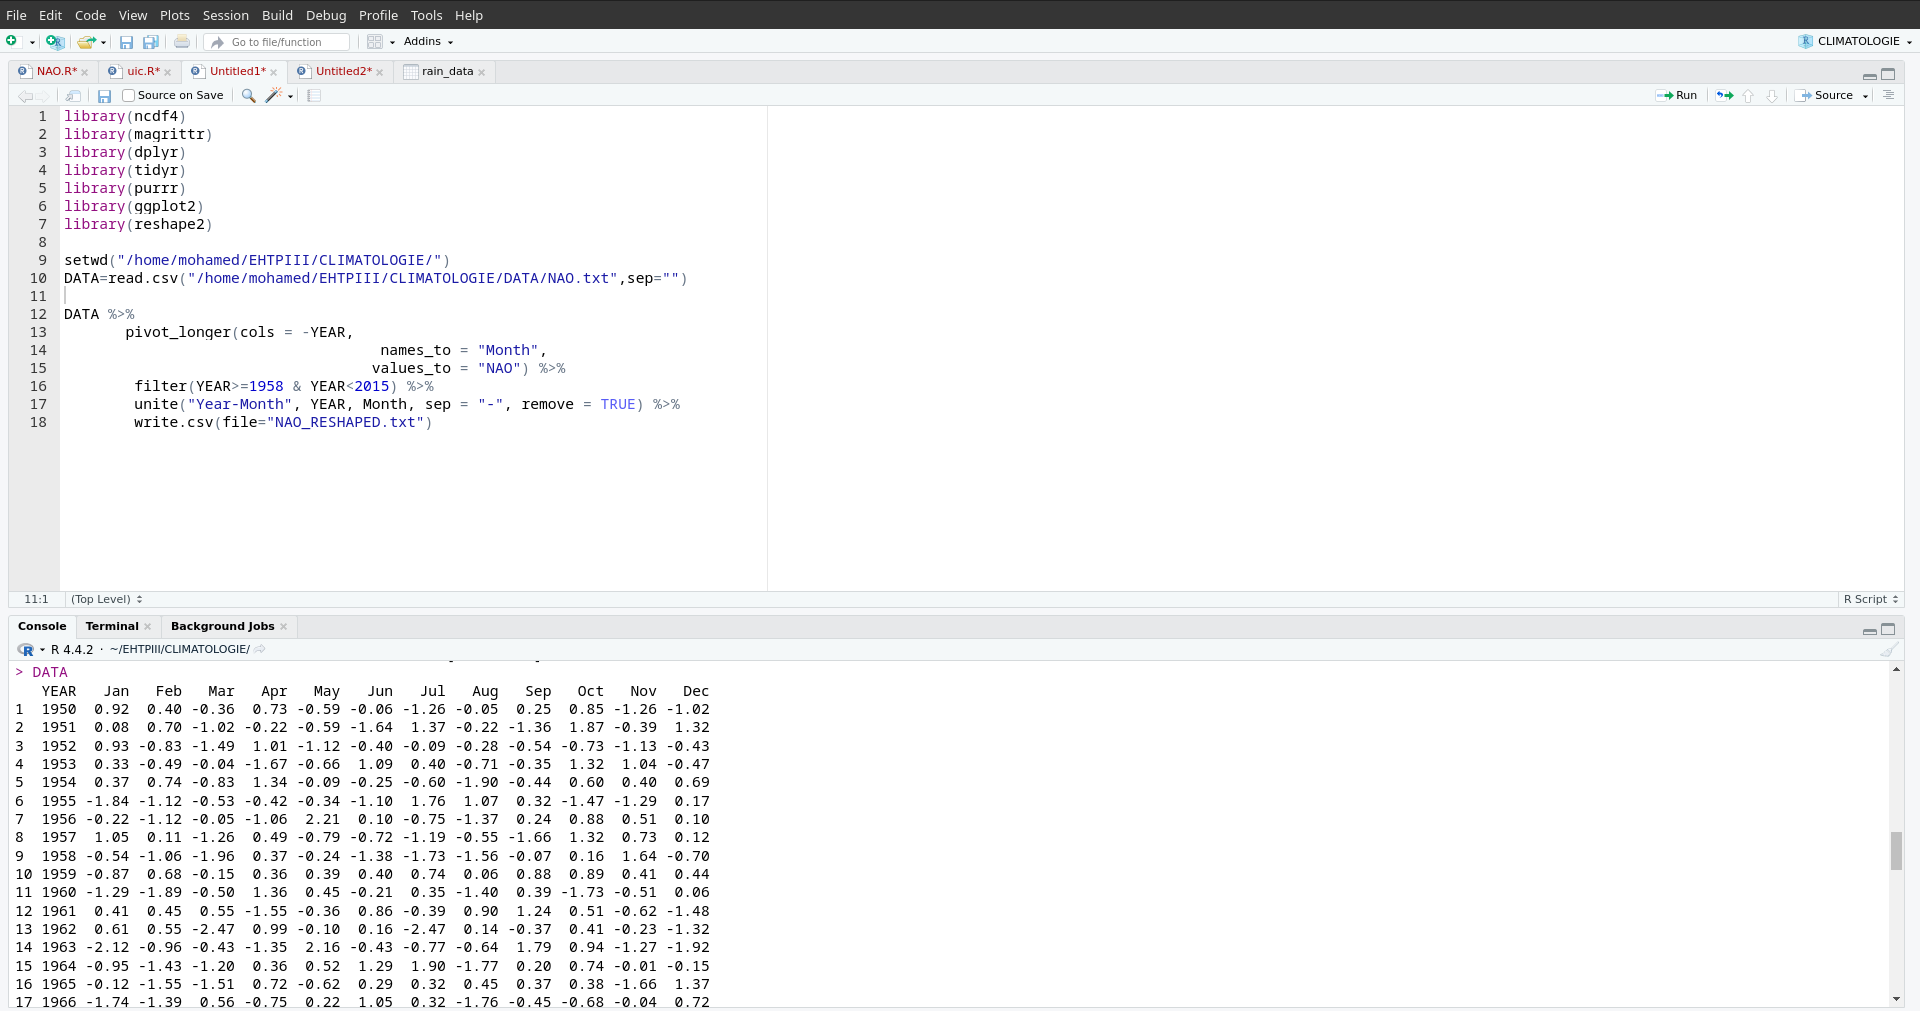
\includegraphics[scale=0.2]{R.png}
\caption{Analyse de données par R}
\end{figure}   
    
    
    \item \textbf{Python} : Utilisé principalement pour le calcul de l'indice d'upwelling en appliquant la méthode de Bakun, en utilisant les données disponibles via la plateforme ERDDAP.

\begin{figure}[H]
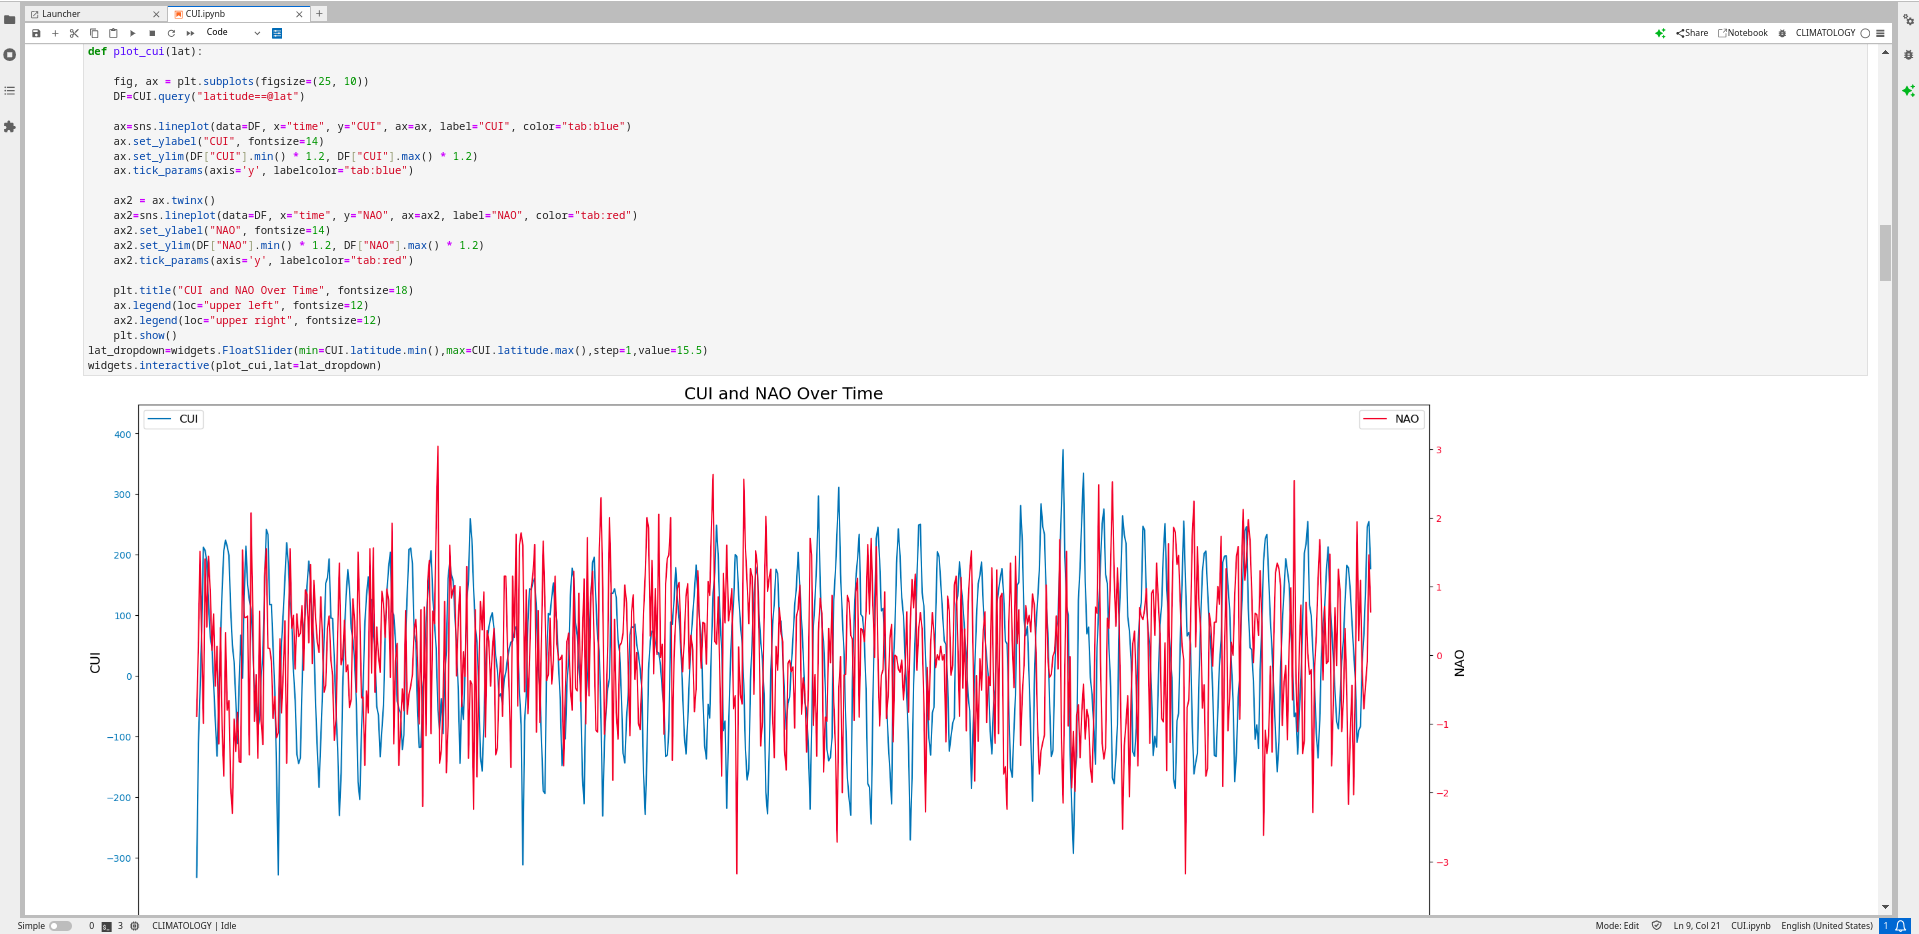
\includegraphics[scale=0.2]{python.png}
\caption{Calcule et Visualisation du CUI par python}
\end{figure}    
    
    
    \item \textbf{CDO (Climate Data Operators)} : Un ensemble d’outils pour la manipulation et l’analyse de données climatiques, particulièrement les fichiers NetCDF.

\begin{figure}[H]
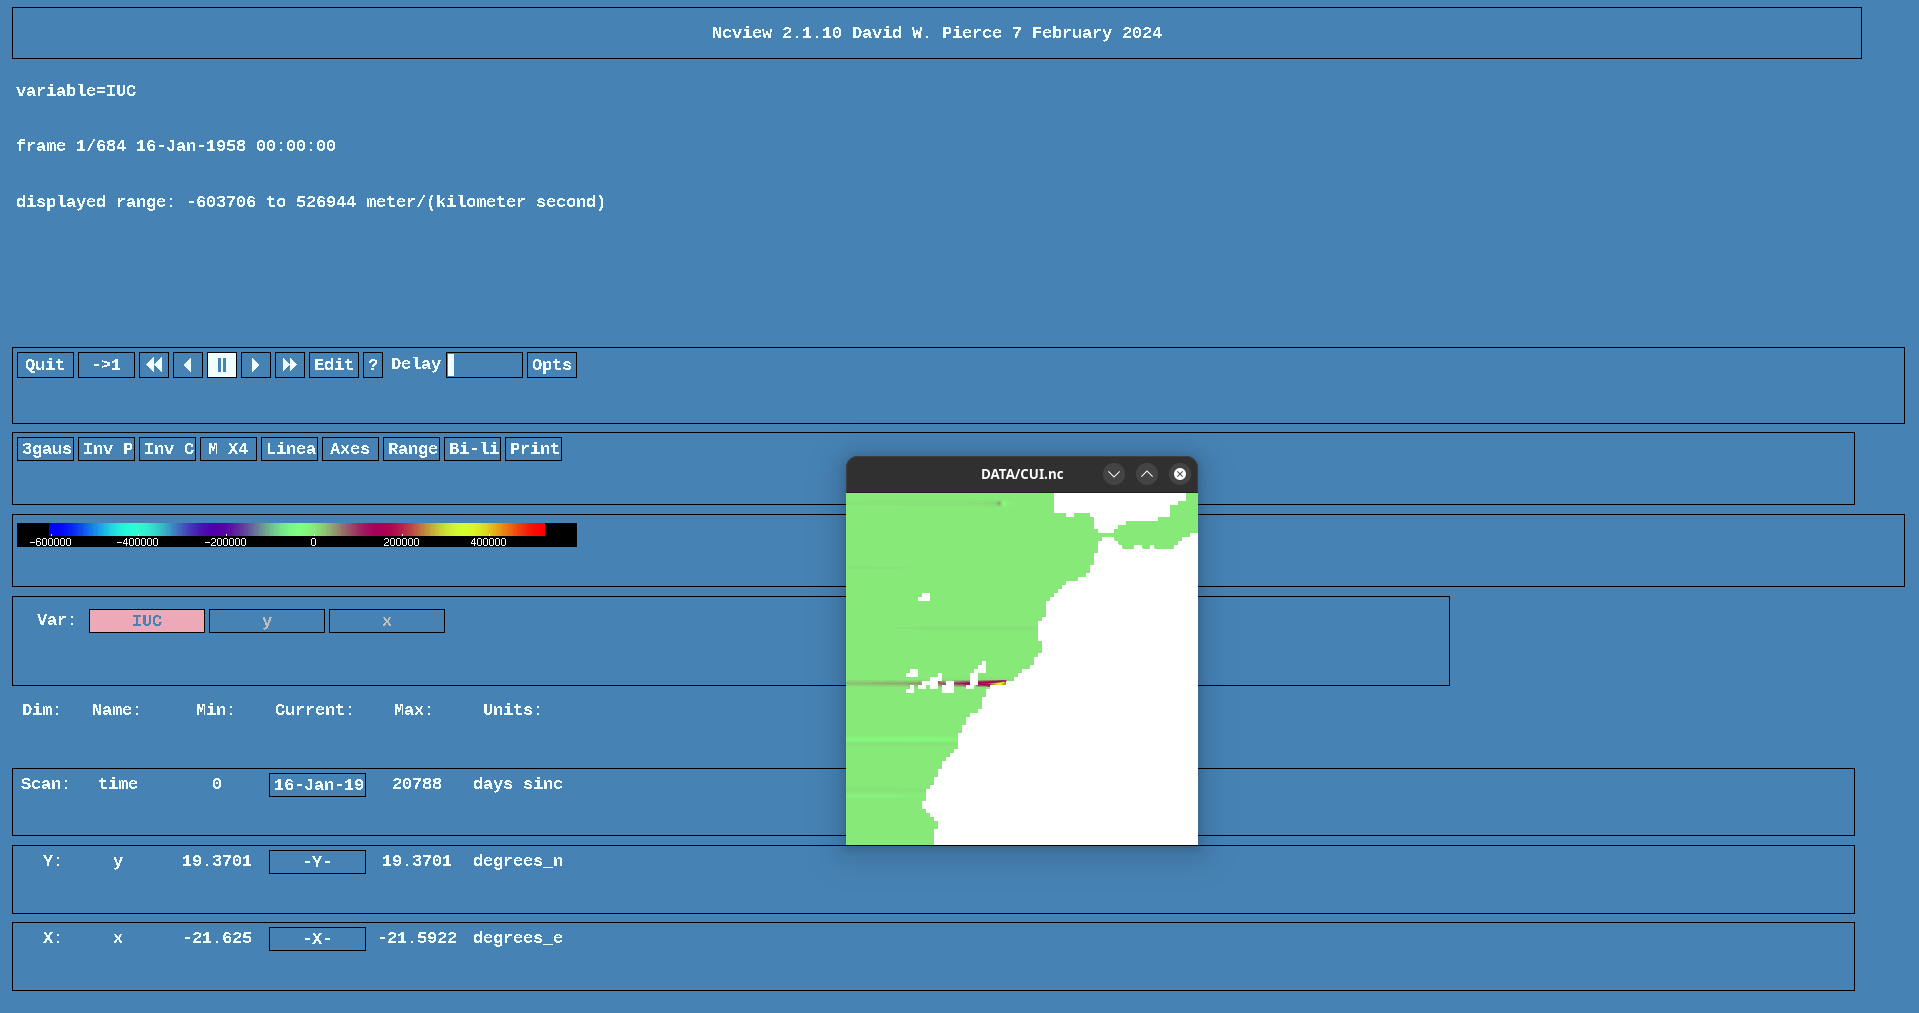
\includegraphics[scale=0.2]{cdo.png}
\caption{Visualisation du CUI sur le Maroc par CDO.}
\end{figure}
    

    
    
    \item \textbf{ERDDAP} : Une plateforme de la NOAA utilisée pour accéder aux données de transport d'Ekman.
\end{itemize}

\subsection{Collecte des données}
\textbf{Les données utilisées pour le calcul de l'indice d'upwelling proviennent principalement de deux sources :} \\

\begin{enumerate}

    \item \textbf{Transport d'Ekman} \footnote{\url{http://coastwatch.pfeg.noaa.gov/erddap/griddap/erdlasFnWPr.html}} : Les composantes $T_x$ (zonale) et $T_y$ (méridienne) du transport d'Ekman pour le Maroc 1950-2022, utilisées pour déterminer la direction de l'upwelling le long de la côte. Ces données sont disponibles via la plateforme ERDDAP de la NOAA.
    \item \textbf{Température de l'océan} \footnote{\url{https://climate.copernicus.eu/climate-reanalysis}} Les réanalyses ERA5 pour la période 1950-2022 avec une fréquence mensuelle, utilisées pour compléter l'analyse des conditions océaniques.
\end{enumerate}
\vspace{1cm}
\textbf{Les données sont structurées sous le format suivant :}
\begin{itemize}
    \item \textbf{time} : Temps, en UTC.
    \item \textbf{latitude} : Latitude en degrés nord 20.5-35.5 ° Nord.
    \item \textbf{longitude} : Longitude en degrés est.
    \item \textbf{pmsl} : Pression au niveau de la mer, en hpa.
    \item \textbf{u\_mean} : Composante zonale du vent, en m/s.
    \item \textbf{v\_mean} : Composante méridienne du vent, en m/s.
    \item \textbf{uv\_mag\_mean} : Magnitude du transport d'Ekman, en m/s.
    \item \textbf{taux\_mean} : Composante zonale du stress du vent, en N/m².
    \item \textbf{tauy\_mean} : Composante méridienne du stress du vent, en N/m².
\end{itemize}

\textbf{L'étendu géographique de la donnée couvre la cote du Maroc  :}

Les données utilisées couvrent les côtes du Maroc, un endroit stratégique pour observer l'upwelling côtier, qui joue un rôle crucial dans la productivité biologique des eaux marocaines.

\subsection{Délimitation de la zone d'étude}
La zone d'étude concerne principalement la façade atlantique du Maroc, s'étendant le long de la côte ouest du pays depuis le détroit de Gibraltar au nord jusqu'au Sahara occidental au sud. Cette région est caractérisée par des conditions climatiques variées influencées par le flux océanique atlantique, les courants marins et les phénomènes de upwelling le long de la côte. L'objectif est d'étudier les interactions entre le North Atlantic Oscillation (NAO) et l'Indice de Remontée côtière (CUI) dans cette région spécifique en analysant les données climatiques et océanographiques.

\begin{figure}[H]
\centering
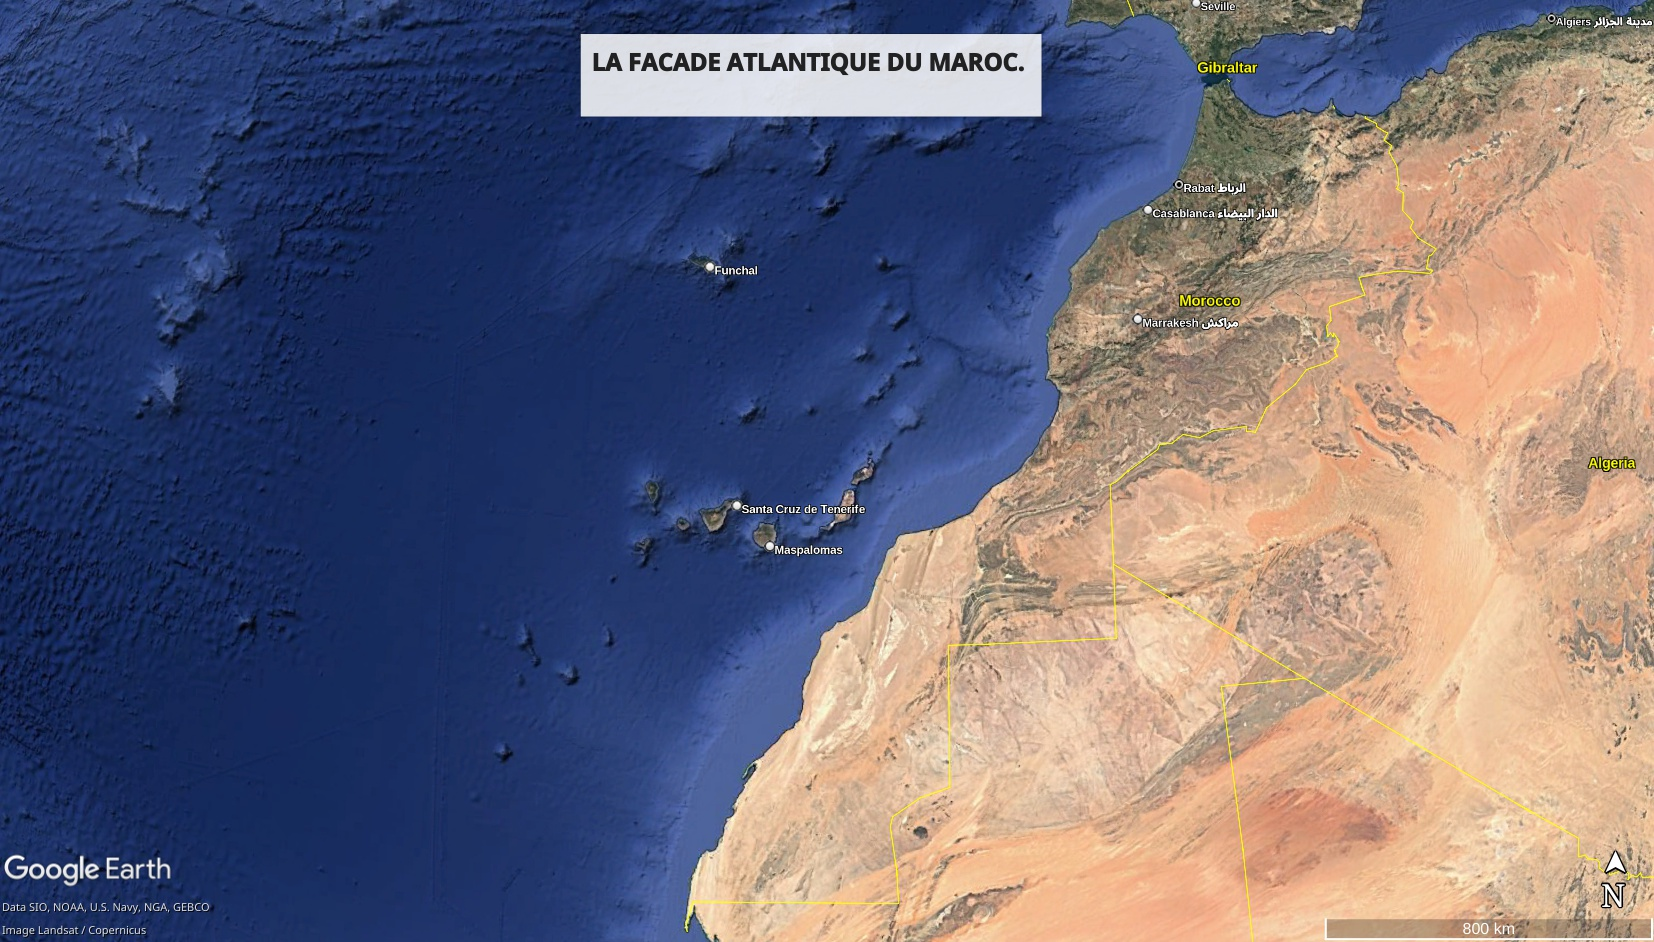
\includegraphics[scale=0.2]{zone.jpg}
\caption{La façade atlantique du Maroc}
\end{figure}




\subsection{Calcul de l'indice d'upwelling de Bakun (CUI)}

L'indice d'upwelling de Bakun (CUI) \footnote{\url{https://www.researchgate.net/publication/252415117_Coastal_Upwelling_Indices_West_Coast_of_North_America_1946-1995}} est calculé en utilisant les composantes $T_x$ et $T_y$ du transport d'Ekman et l'orientation de la côte. La formule utilisée pour déterminer l'intensité de l'upwelling est la suivante :

\[
CUI = \frac{T_x \cos(\alpha) + T_y \sin(\alpha)}{10}
\]

où :
\begin{itemize}
    \item $T_x$ : Composante zonale ($x$) du transport d'Ekman en \textit{m/s}.
    \item $T_y$ : Composante méridienne ($y$) du transport d'Ekman en \textit{m/s}.
    \item $\alpha$ : Orientation de la côte par rapport au nord géographique en degrés.
\end{itemize}

Le facteur 10 est utilisé pour normaliser les valeurs de l'indice, afin d'obtenir des résultats compatibles avec les études précédentes et pour simplifier l'interprétation de l'intensité de l'upwelling. 

\subsubsection{Description de la fonction Python pour le calcul du CUI}

La fonction Python utilisée pour calculer l'indice d'upwelling, en prenant en entrée les composantes du transport d'Ekman et l'angle d'orientation de la côte, est la suivante :

\begin{verbatim}
def upwell(ektrx, ektry, coast_angle):
    import numpy as np
    pi = 3.1415927
    degtorad = pi/180.
    alpha = (360 - coast_angle) * degtorad
    s1 = np.cos(alpha)
    t1 = np.sin(alpha)
    s2 = -1 * t1
    t2 = s1
    perp = (s1 * ektrx) + (t1 * ektry)
    para = (s2 * ektrx) + (t2 * ektry)
    return(perp/10)
\end{verbatim}

\subsection*{ Explication du code} :
\textbf{\textit{Entrées de la fonction}} : \\
   \begin{itemize}
       \item \texttt{ektrx} : Composante zonale ($T_x$) du transport d'Ekman en \textit{m/s}.
       \item \texttt{ektry} : Composante méridienne ($T_y$) du transport d'Ekman en \textit{m/s}.
       \item \texttt{coast\_angle} : Orientation de la côte par rapport au nord géographique en degrés.
   \end{itemize} 
   
\textbf{\textit{Calcul de l'angle $\alpha$}} : \\ 
   \[
   \alpha = (360 - \text{coast\_angle}) \times \frac{\pi}{180}
   \] 
   
   
L'orientation de la côte est entrée sous forme d'un "angle de côte", qui est l'angle que fait la côte par rapport au nord dans le sens mathématique. Cet angle est défini comme l'angle que le côté terrestre de la côte forme avec un vecteur pointant vers le nord, comme illustré dans les images suivantes, où l'angle $\alpha$ (alpha) représente l'"angle de côte". 
\vspace{0.5cm}

Cet angle $\alpha$ est mesuré en degrés dans le sens horaire à partir du nord géographique. Par exemple, pour une côte orientée nord-sud, l'angle de côte $\alpha$ serait de $90^\circ$. Une côte orientée sud-ouest/nord-est aurait un angle d'environ $\alpha \approx 135^\circ$.

\begin{figure}[H]
\centering
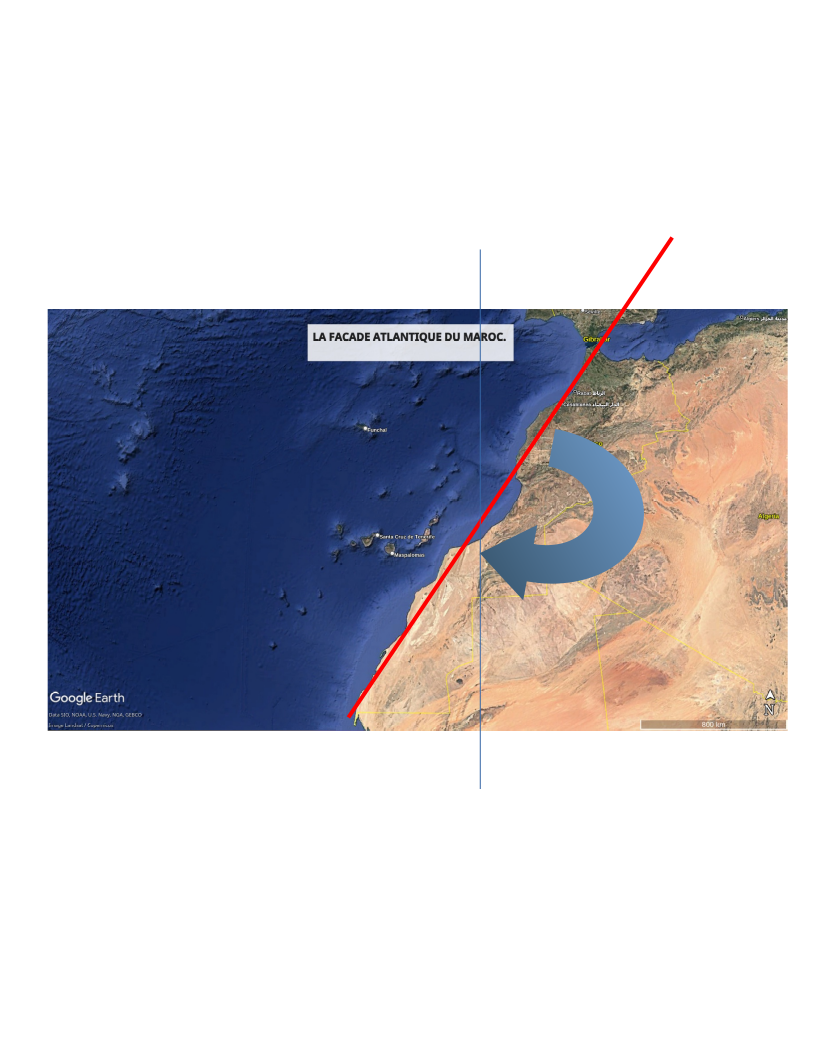
\includegraphics[scale=0.5]{angle.png}
\caption{l'angle $\alpha$ pour le Maroc}
\end{figure}

Pour la côte marocaine, l'orientation générale varie selon les différentes régions, mais en moyenne, l'angle de côte pour la majorité de la côte atlantique et méditerranéenne du Maroc est d'environ $\alpha \approx 135^\circ$, ce qui correspond à une orientation sud-ouest/nord-est.
\vspace{1cm}


\textbf{\textit{Calcul des composantes perpendiculaires et parallèles}} : \\
   \begin{itemize}
       \item \texttt{s1} et \texttt{t1} sont les composantes du vecteur unité dans la direction perpendiculaire à la côte.
       \item \texttt{s2} et \texttt{t2} sont les composantes du vecteur dans la direction parallèle à la côte.
   \end{itemize}

\textbf{\textit{Calcul du transport d'Ekman perpendiculaire et parallèle}} : \\
   Le transport d'Ekman perpendiculaire à la côte (pour l'upwelling) est calculé comme :
   \[
   \text{perp} = (s1 \times \text{ektrx}) + (t1 \times \text{ektry})
   \]
   La composante parallèle n'est pas utilisée pour le calcul du CUI, mais elle est calculée pour des analyses complémentaires.


\textbf{\textit{Retour de l'indice CUI normalisé}} : \\
   L'indice CUI est donné par la composante perpendiculaire divisée par 10 pour normalisation :
   \[
   CUI = \frac{\text{perp}}{10}
   \]






\subsection{Importance de l'indice CUI}

L'indice CUI est crucial pour comprendre l'intensité de l'upwelling côtier, un phénomène clé pour la productivité biologique dans les zones côtières. Il est particulièrement utile pour surveiller les changements dans les écosystèmes marins et pour analyser les impacts du climat et des conditions atmosphériques sur la dynamique océanique.



\subsubsection{Sélection des points significatifs}
Une fois les valeurs du CUI calculées pour l'ensemble des points le long de la côte marocaine, une sélection des zones les plus pertinentes a été effectuée. Ces zones correspondent aux points où l'intensité de l'upwelling est la plus importante. La sélection repose sur des critères géographiques et physiques, tels que la bathymétrie et l’exposition côtière, afin de s’assurer que les résultats sont représentatifs des processus océanographiques régionaux.

les points sélectionnés sont représentés par les latitudes de 20.5 à 36.5 ° N.


\subsection{Synthèse des outils et flux de travail}
L'approche globale s'articule autour des étapes suivantes :
\begin{enumerate}
    \item Collecte des données climatiques via ERDDAP (transport d'Ekman) et ERA5 (température).
    \item Prétraitement des données avec \textbf{CDO} (interpolation, extraction des régions d'intérêt).
    \item Calcul des indices CUI à l'aide de \textbf{Python}.
    \item Analyse statistique et visualisation des résultats dans \textbf{R}.
\end{enumerate}
Ce flux de travail garantit une cohérence entre les différentes étapes de traitement et permet une analyse robuste et reproductible.
